\section{Experimental Details}
	The experiment was carried out with utmost care, following the radiation safety guidelines. The surroundings of the path of the photons radiated from the gamma radiation sources were carefully obstructed and the experiment area was checked with a Geiger counter before anyone interacted with the setup. 
	\\
	\\
	The procedure consisted of two parts that will be explained individually later in this section. The experiment took approximately two hours including the two procedures, discussion about the experiment with the TA and necessary calculations.
	\\
	\\
	The experiment setup used can be seen in the figure below, the equipment will be explained individually.
	
	\begin{figure}[h]
		\caption{Experiment Setup}
		\centering
		\label{fig:ExperimentSetup}
		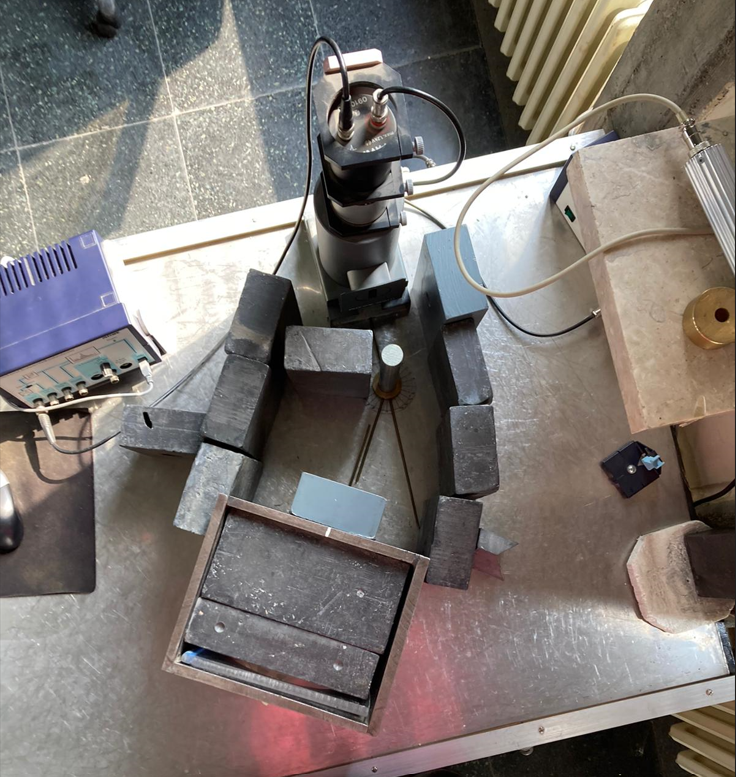
\includegraphics[width=\textwidth / 2]{images/exp_setup.png}
	\end{figure}

	\subsection{Equipment}
		
		\subsubsection{Multi Channel Analyzer}
		A multichannel analyzer is an instrument that uses a fast analog to digital converter to analyze incoming input pulses and is a popular instrument used in gamma spectroscopy. The data taken from the MCA will be presented in the next section.
		
		\begin{figure}[h]
			\caption{The Multi Channel Analyzer Used In The Experiment}
			\centering
			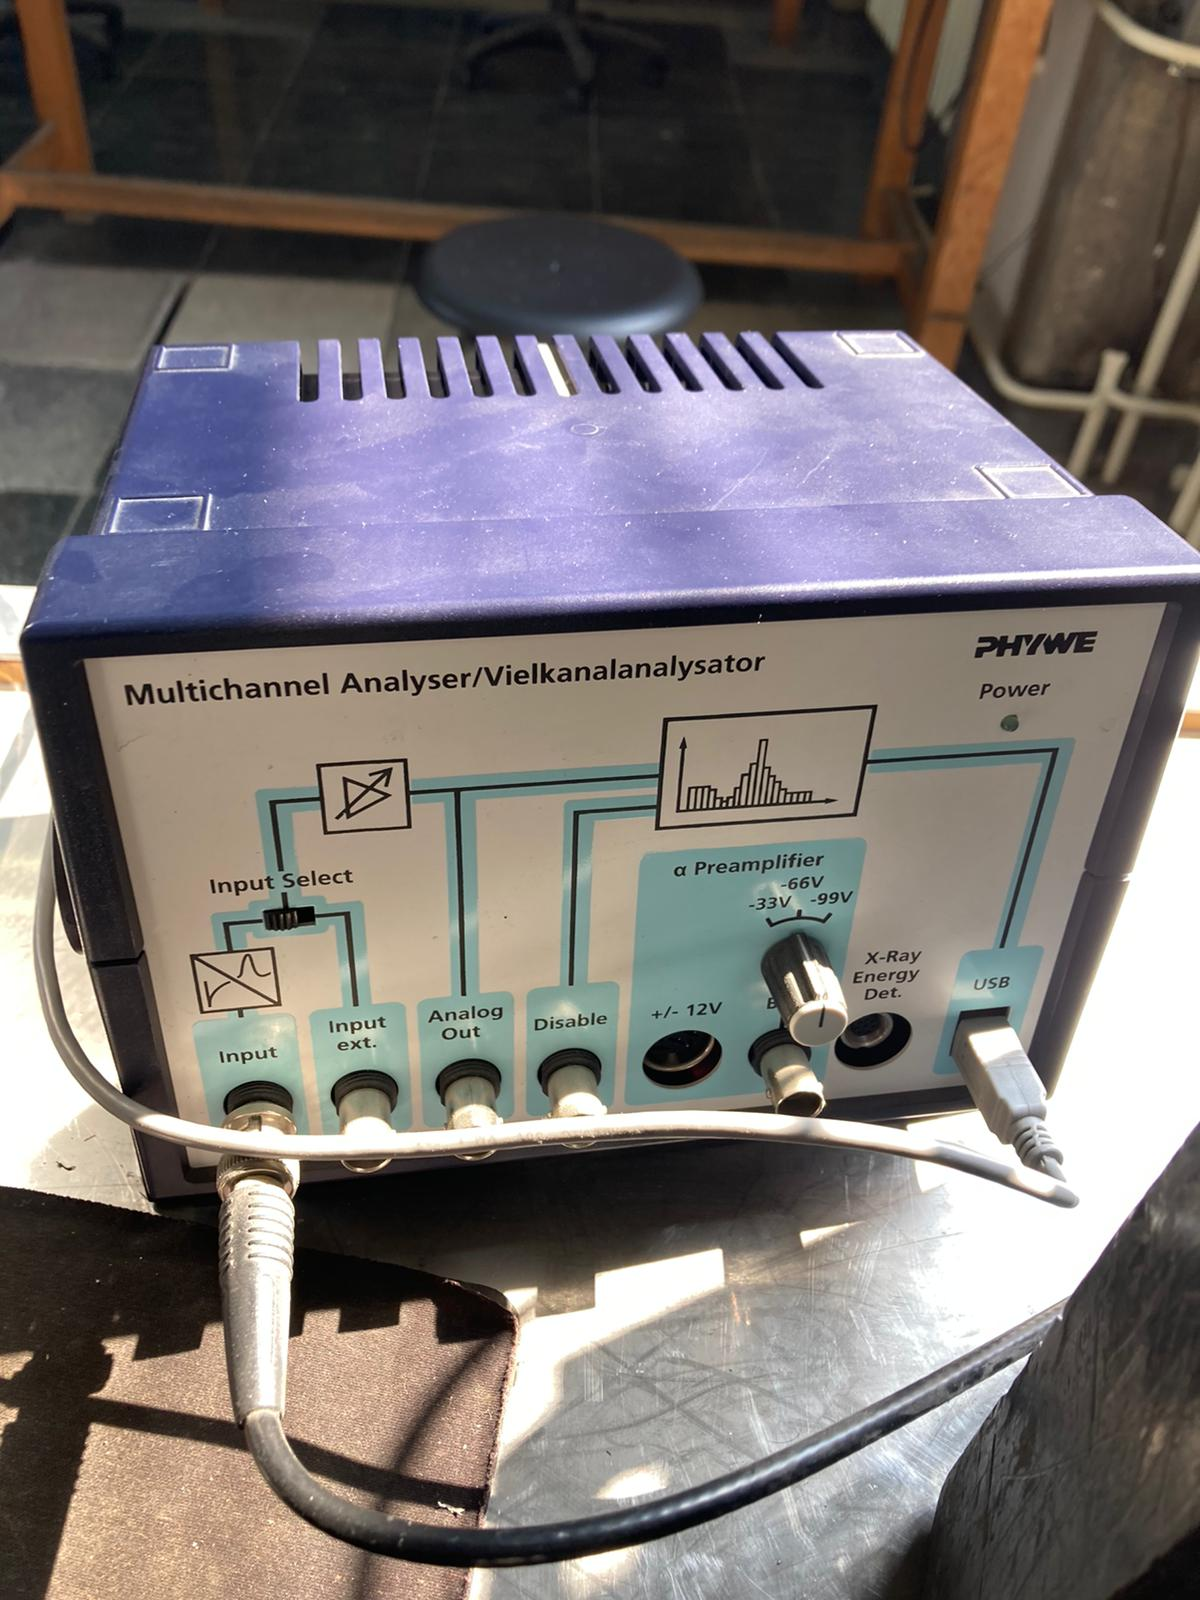
\includegraphics[width=\textwidth / 2]{images/mca.jpeg}
		\end{figure}
		
		\subsubsection{Radioactive Source}
			
			Two radioactive sources were used during the experiment.
			
			\paragraph{CS - 137, 37 kBq}
			This source was encased in a small lead block and used during the calibration process. Its small size allowed it to be  around safely without much effort. When the calibration process was over, this source was carefully removed from the setup and left adjoining the wall.
			
			\paragraph{CS - 137, 18.5 MBq}
			This source was encased in a large lead block, had wheels attached to it and used during the experiment procedure. A thick lead block was present in front of this source during the calibration process for safety reasons, the block was only removed briefly for the experiment procedure. The source is encased in the large lead block which can be seen in Figure \ref{fig:ExperimentSetup}.
		
		\subsubsection{Gamma Detector}
			The gamma detector used in this experiment is a scintillation counter, which consists of a scintillator crystal and a photomultiplier tube connected to it.
			\paragraph{Scintillator}
				Scintillators absorb incoming particles (or ionizing radiation, ie. gamma radiation used in this experiment) to emit the absorbed energy as light. Scintillators themselves work on the principle of Compton effect, which is a nice correlation.
				\begin{figure}[h]
					\caption{A Scintillator Crystal}
					\centering
					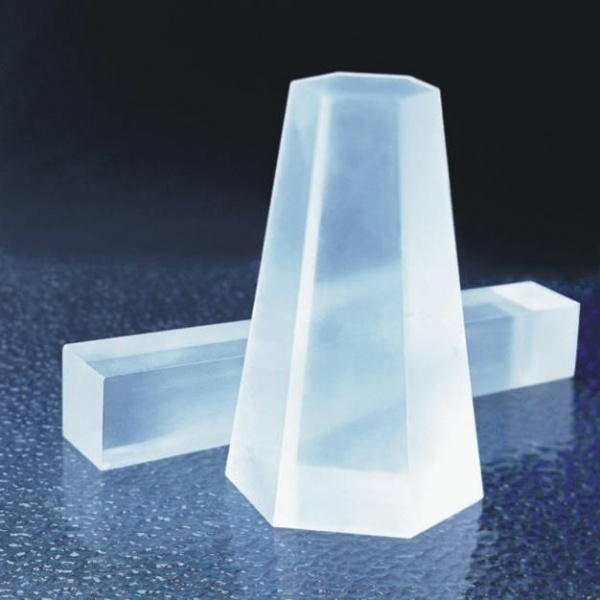
\includegraphics[width=\textwidth / 2]{images/scintillator.jpg}
				\end{figure}
			
			\paragraph{Photomultiplier Tube}
				A photomutiplier tube allows the incoming photons to hit the photocathode material inside, allowing electrons to eject its surface because of photoelectric effect. The ejected electrons are then directed over to the electron multiplier where secondary emission allows the electrons to be multiplied.
			
				\begin{figure}[h]
					\caption{Photomultiplier Tube Schematic}
					\centering
					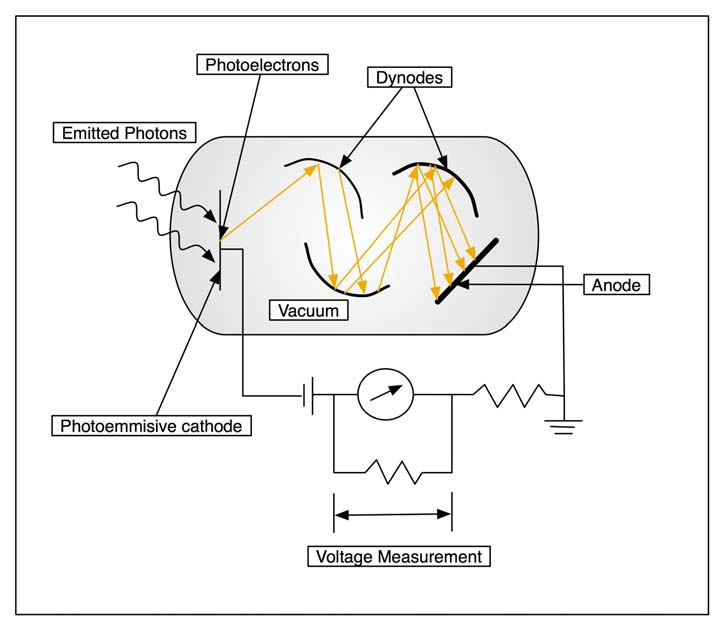
\includegraphics[width=\textwidth / 2]{images/pmt.png}
				\end{figure}
			
			\paragraph{Operating Unit}
				The operating unit of the detector is rsponsible for supplying the appropriate voltage in a stable way to the photomultiplier tube. It operates between 600 Volts and 1100 Volts.
				\\
				\\
				During the experiment, the voltage knob was at the scale 8.00, which corresponds to 1000 Volts.
		
		\subsubsection{Iron Rod}
			An iron rod is used as an electron source in this experiment. The photons radiated by the gamma source hit the iron rod and scatter photons to be detected by the detector.
		
		\subsubsection{Lead Block}
			Several lead blocks are used in the experiment for safety reasons. Everywhere except the direct path of the incident radiation is obstructed by lead blocks, which in turn has consequences in the measured result which will be discussed in the discussion section.
	
	\subsection{Procedure}
	
		\subsubsection{Calibration Procedure}
			The calibration process was performed as follows:
				\begin{itemize}
					\item The MCA was turned on and its proprietary software was set up to make measurements.
					\item The voltage knob of the operating unit of the detector was adjusted to the scale value of 8.00 to supply the necessary voltage to the detector. 
					\item Cs - 137, 37kBq, which is the source encased in the smaller lead block, was carefully inserted in front of the detector, adjoining it. 
					\item The calibration process was started in the software.
					\item Waited around 15 - 20 minutes for the measurements.
					\item Analyzed the resulting spectra with the TA.
					\item Identified the two sharpest peaks corresponding to two different types of radiation from the source and marked them.
					\item Assigned known peak values for Cs - 137 to the marked peaks, completing the calibration process.
					\item The calibration was saved on the software and the radiation source was carefully removed.
				\end{itemize}
		
		\subsubsection{Experiment Procedure}
			The experiment procedure was performed as follows:
				\begin{itemize}
					\item The software was set up to make measurements again. 
					\item The iron rod, which acts as an electron source, was inserted in front of the larger gamma source and its angle was arranged with an old and worn down instrument.
					\item The direct path of the radiation was blocked by a lead block to ensure that we mostly measure the radiation due to Compton scattering.
					\item The lead cover of the Cs - 137, 18.5 MBq source was carefully removed to let radiation hit the iron rod.
					\item The measurements was started with the software.
					\item Waited around 15 - 20 minutes one again for the measurements.
					\item After we had enough data, the lead cover of the radiation source was carefully inserted in front of it once again and the measurement process was done.
					\item The resulting spectra was analyzed with the TA and had verbal discussion on it.
					\item Performed smoothing on the measured data and saved the plots for the laboratory report.
				\end{itemize}
